% Unofficial International Conference on Travel Behavior Research (IATBR) Conference template
% Based on the proposed Word template available at:
%https://view.officeapps.live.com/op/view.aspx?src=https%3A%2F%2Fiatbr2024.univie.ac.at%2Ffileadmin%2Fuser_upload%2Fk_iatbr2024%2Fiatbr2024_template_example.docx&wdOrigin=BROWSELINK

% This template is unofficial, free, and comes with ABSOLUTELY NO WARRANTY. You are welcome to redistribute it.

% Version 1.0
% Santiago Álvarez-Ossorio Martinez, Technical University of Munich, Chair of Traffic Engineering and Control
%   1.0   - August 2023

\documentclass[12pt]{article}
\usepackage[utf8]{inputenc}
\usepackage{tikz}
% \documentclass{article}
\usepackage{algorithm}
\usepackage{algpseudocode}
\usetikzlibrary{positioning}
\usetikzlibrary{shapes,arrows,arrows,positioning,fit}

% Required Packages
\usepackage{fancyhdr} % Headers and footers
\usepackage{xcolor, soul} % Colors + Highlighting using \hl{}
\usepackage{lipsum} % To generate dummy text
\usepackage{times} % Times New Roman Font
\usepackage[left=3cm, right=3cm, top=2.5cm, bottom=2.5cm]{geometry} % Page dimensions
\usepackage{graphicx}
\usepackage{caption}
\usepackage{subcaption}
\usepackage{float}
\usepackage{orcidlink} % To inclue the ORCID link and logo
\usepackage{amsmath} % For formulae
\usepackage{array} % For table styling
\usepackage{tabularx}
\sethlcolor{yellow}

% For tables (optional)
\usepackage{longtable}
\usepackage{dcolumn}
\newcolumntype{d}[1]{D{.}{.}{#1}}
% Typesetting-quality tables, rules in tables (\toprule, \midrule)
\RequirePackage{booktabs}
% tables (after hyperref):
\RequirePackage{tabularx}
\RequirePackage{xparse}
\RequirePackage{totcount}
\usepackage{parskip}
\usepackage{hyperref}

%%%%%%%%%%%%%%%%%%%%%%%%%%%%%%%%%%%%%%%%%%%%%%%%%%%%%%%%%%%%%%%%%%%%
%%%%%%%%%%%%%%% TEMPLATE AND FORMATING %%%%%%%%%%%%%%%%%%%%%%%%%%%%%
%%%%%%%%%%%%%%%%%%%%%%%%%%%%%%%%%%%%%%%%%%%%%%%%%%%%%%%%%%%%%%%%%%%%

% For APA citation style
% \usepackage[style=apa, backend=biber, sorting=nyt]{biblatex}
% \DeclareLanguageMapping{english}{english-apa} % required for biblatex-apa
% \addbibresource{references.bib} % Linking to the .bib file

% uniquelist=false -> + Info in https://tex.stackexchange.com/questions/121625/biblatex-modify-maxcitenames-to-work-in-three-cases -> Used to avoid having more than one author name in the citation when there are several cited papers that share some (but not all) authors.
\usepackage[maxcitenames=1, mincitenames=1, authordate,bibencoding=auto,strict,backend=biber,natbib, dashed=false,uniquelist=false]{biblatex-chicago}

\addbibresource{references.bib} % Linking to the .bib file

% For Custom IATBR citation style
% Define custom citation commands
\DeclareCiteCommand{\citeintext}
  {\boolfalse{citetracker}%
   \boolfalse{pagetracker}%
   \usebibmacro{prenote}}
  {\ifciteindex
     {\indexnames{labelname}}
     {}%
   \printnames{labelname}%
   \setunit{\nameyeardelim}%
   (\usebibmacro{citeyear})}
  {\multicitedelim}
  {\usebibmacro{postnote}}

\renewbibmacro*{in:}{} % Removes "In:"

\newcolumntype{Y}{>{\centering\arraybackslash}X} % For custom centered cells in tabularx

% Set page style to fancy and clear all headers/footers
\pagestyle{fancy}
\fancyhf{}
\renewcommand{\headrulewidth}{0pt} % Removes the line below the header

% Adjust distance of the header from the top of the page
\setlength{\headsep}{1.25cm}

% Adjust the footskip value for page numbering distance from the bottom
\setlength{\footskip}{1.0cm}

\setlength\parindent{0pt} % To avoid indenting og the first line of each paragraph that doesn't immediately follow a section heading (IATBR word template does not have such indentation)

% Header with the conference name in gray
% \chead{{\color[HTML]{C0C0C0}\fontsize{12}{14}\selectfont 17th International Conference on Travel Behaviour Research\\ July 14 - 18, 2024 – Vienna, Austria
% }}

% Page numbering in gray
\cfoot{{\color[HTML]{C0C0C0}\thepage}}

% Title, Author, and Affiliation Definitions
\newcommand{\doctitle}[1]{{\centering \fontsize{20}{22}\selectfont \textbf{#1} \par}}
\newcommand{\docauthor}[1]{{\centering \fontsize{14}{16}\selectfont \textbf{#1} \par}}
\newcommand{\docaffiliation}[1]{{\centering \fontsize{12}{14}\selectfont #1 \par}}

\newcommand{\dockeywords}[1]{{\fontsize{12}{14}\selectfont \textbf{Keywords :} #1 \par}}


% Redefine section to follow the required format with an indentation
\makeatletter
\renewcommand\section{\@startsection {section}{1}{1em}%
                                   {-3.5ex \@plus -1ex \@minus -.2ex}%
                                   {2.3ex \@plus.2ex}%
                                   {\normalfont\fontsize{14}{16}\bfseries}}
\renewcommand{\thesection}{\arabic{section}.}

\renewcommand\subsection{\@startsection {subsection}{2}{1em}%
                                   {-3.25ex \@plus -1ex \@minus -.2ex}%
                                   {1.5ex \@plus .2ex}%
                                   {\normalfont\fontsize{12}{14}\bfseries}}
\renewcommand{\thesubsection}{\thesection\arabic{subsection}}
\makeatother

%%%%%%%%%%%%%%%%%%%%%%%%%%%%%%%%%%%%%%%%%%%%%%%%%%%%%%%%%%%%%%%%%%%%
%%%%%%%%%%%%%%% CONTENT OF THE PAPER %%%%%%%%%%%%%%%%%%%%%%%%%%%%%%%
%%%%%%%%%%%%%%%%%%%%%%%%%%%%%%%%%%%%%%%%%%%%%%%%%%%%%%%%%%%%%%%%%%%%

\begin{document}

% Title, Author, and Affiliation
\doctitle{Spotted Hyena Optimization}
\hfill\break%
\docauthor{Yogesh Shinde\textsuperscript
           }
\docaffiliation{Indian Institute of Information Technology(IIIT), Dharwad \\20bds065@iiitdwd.ac.in\\}
\hfill
\vspace{5pt}
\hrule
\vspace{5pt}
\textbf{\large{Abstract}}\\
\\
A Spotted hyena Optimization (SHO) is nature inspired optimization algorithm which try to mimic the hunting pattern of spotted hyenas.
Spotted hyena Optimization (SHO) is a metaheuristic algorithm,  which is inspired by social hierarchy and collaborative hunting behavior of spotted hyenas. It can be categorized as a swarm-based algorithm.
So searching for prey, encircling the prey, and attack on prey are the 3 basic steps of SHO.
It is simple to implement and efficient, and it has been shown to be effective in solving a variety of engineering optimization problems. It is particularly good at finding solutions to problems with a large number of variables.
This paper carries out a comprehensive review of SHO, in order to apply it to real life engineering problems. 
However, it also motivates new researchers and algorithm creators to better understand and utilize this straightforward yet highly effective method for solving problems.
\\
\\
\textbf{Keywords : }Spotted Hyena Optimization Algorithm, Optimization techniques, Meta heuristics.\\

\vspace{7pt}
\hrule


% Sample sections and content
\section{Introduction}
In recent times, the increasing complexity of real-world problems has led to a growing demand for enhanced metaheuristic techniques. These methods are invaluable for obtaining optimal solutions in the context of engineering design challenges, gaining popularity due to their efficiency and versatility when compared to conventional classical approaches. Metaheuristic optimization algorithms are a class of population-based stochastic algorithms that are designed to solve complex optimization problems. They have been successfully applied to a wide variety of problems in engineering, science, and business. In recent years, there has been a growing interest in the development of new metaheuristic algorithms inspired by nature. One such algorithm is the Spotted Hyena Optimizer (SHO) (\cite{dhiman2017spotted}).

Metaheuristic approaches can be broadly categorized into three main groups: evolutionary-based, physical-based, and swarm-based methods. 
Evolutionary-based methods, like Genetic Algorithms (GA) ( \cite{mirjalili2019genetic}) and Differential Evolutionary , simulate the process of biological evolution, evolving populations of solutions over generations, commonly applied to optimization problems such as parameter tuning in machine learning. 
Physical-based methods, such as Simulated Annealing (SA) , model natural phenomena or physical processes, with particles moving through a search space and adjusting their positions based on experiences, used in optimization and control tasks. Other famous Physical-based methods include Harmony Search. 
Swarm-based methods, like Ant Colony Optimization (ACO) and Particle Swarm Optimization (PSO), draw inspiration from collective behaviors in social or biological systems, where groups of agents collaborate towards a common goal, often employed in solving routing or scheduling problems.
Other popular swarm intelligence techniques are, Cuckoo Search (CS) (\cite{yang2010engineering}), Firefly Algorithm (FA) (\cite{yang2010firefly} )etc.

Using a single optimizer to tackle various optimization problems with different characteristics doesn't ensure success. This idea has inspired to develop a novel metaheuristic algorithm called Spotted Hyena Optimization (SHO) [1], which takes its inspiration from the world of biology. 
The SHO is a new bio-inspired technique that draws its inspiration from the teamwork and hunting strategies observed in spotted hyenas. Similar to how spotted hyenas work together efficiently in cohesive groups, it uses clustering to enhance cooperation among its components. 
The SHO algorithm's key steps are influenced by the way these animals hunt. In a rigorous evaluation, it's effectiveness is tested on a set of challenges. 
The outcomes highlight SHO's superior performance when compared to other competing algorithms in the proposed paper.   
So in this paper we will review the same algorithm and analyze its performance over standard problems to optimize it.

In this paper, we present a review of the Spotted Hyena Optimizer (SHO) algorithm. We discuss the algorithm's motivation, design, implementation, and evaluation. We also discuss the algorithm's limitations and future research directions. We believe that the SHO algorithm is a promising new metaheuristic algorithm with the potential to be applied to a wide variety of optimization problems. We hope that this paper will provide a useful overview of the algorithm and encourage further research in this area. The structure of this paper can be outlined as follows: In Section 2 is dedicated to literature search. Coduct a comparative analysis with existing literature to establish the effectiveness of the SHO approach. Moving on to Section 3, it briefly presents the SHO algorithm and methodology employed. 
In Section 4, we comprehensively discuss the simulation and experimental results achieved through the implementation of the SHO method. 
Section 5 concludes the insights and important findings from the analysis.

% [[This unofficial IATBR 24 \LaTeX~template replicates the suggested Word template provided in \href{https://iatbr2024.univie.ac.at/abstract-submission/}{the conference's website}. An example of an in-text citation could be \citet{Garrow2009}. Multiple in-text citations are supported, as \citet{Bierlaire2003,Koppelman2005}. Parenthetical citations are also possible~\citep{Bierlaire2003}.
% ]]



\section{Literature Review}

The original work on the SHO algorithm was published in 2017 by Gaurav Dhiman and Vijay Kumar (\cite{dhiman2017spotted}). The paper proposes the algorithm and evaluates its performance on a set of benchmark test functions and five real-life engineering design problems. The results show that the SHO algorithm is competitive with other existing metaheuristic algorithms. Further advancement and use of SHO was explored in the next paper by the same author (\cite{dhiman2017spotted,dhiman2018multi}) Since the original paper was published, there have been a number of studies that have proposed improvements and extensions to the SHO algorithm. These studies have focused on improving the algorithm's performance, robustness, and scalability.

In the original SHO algorithm, the learning rate is a constant value. However, a number of studies have proposed using an adaptive learning rate, which can improve the algorithm's performance. For example, the adaptive learning rate that is based on the number of iterations ( \cite{ghafori2021advances}) The SHO algorithm is a population-based algorithm, and the diversity of the population is important for its performance. A number of studies have proposed techniques for improving the diversity of the SHO algorithm. technique proposed in (2020) for introducing diversity into the population by randomly swapping solutions between different hyenas. (\cite{kumar2020binary,dhiman2019spotted}) The study by by Dhiman (\cite{dhiman2017spotted,dhiman2018multi}), proposed a multi-objective SHO algorithm that uses a Pareto-based selection mechanism. SHO algorithm can be hybridized with other metaheuristic algorithms like Particle Swarm Optimization algorithm to improve its performance. The SHO algorithm has been applied to a variety of optimization problems, including engineering design, scheduling, and financial optimization. The results of these studies have shown that the SHO algorithm is a promising new algorithm for solving a wide range of optimization problems.
 The SHO algorithm has been applied to machine learning problems, such as the training of neural networks (\cite{ghafori2021advances,ewees2021new}) and the tuning of hyperparameters and feature selection (\cite{kumar2020binary,luo2021using}). It is used in financial optimization problemslike portfolio optimization problem. The neural network and image processing problems uses SHO for solving problems like image segmentation and image denoising. The SHO algorithm is a relatively new algorithm, and its applications are still being explored. However, the studies that have been conducted so far have shown that the SHO algorithm has the potential to be applied to a wide range of optimization problems.

 There is still room for improvement in the performance of the SHO algorithm. Researchers are working on developing new techniques to improve the algorithm's convergence rate and its ability to find the global optimum. 
 The SHO algorithm is still sensitive to the parameter settings. It can be computationally expensive for large-scale problems. 
 The theoretical properties of the SHO algorithm are still not well understood. Researchers are working on developing a better understanding of the algorithm's behavior. The literature survey shows that there is a growing interest in the algorithm, and there is a lot of ongoing research on improving its performance and applications.

 




\section{Methodology}
% \lipsum[7-9]
Spotted hyenas are big meat-eating animals that live in dry, open places. They eat animals like zebras, impalas, and wildebeests, which come in different sizes. Spotted hyenas are smart and social creatures. They can recognize their family members using their senses, and they have a social hierarchy. When they hunt together as a group, they are quite successful in catching prey in the wild. Spotted Hyena Optimization (SHO) works a bit like how a group of spotted hyenas hunt together in the wild. Just like hyenas work as a team, SHO uses teamwork to solve problems. 
It has different steps, just like how hyenas have steps in their hunting. Figure 1 shows the different phases of spotted-hyena hunting behavior, first of all the searching and tracking prey then chasing, troublesome and encircling and lastly immobilizing and attacking the prey.
So in implementation first, it looks for possible solutions to the problem, like how hyenas look for prey. 
Then, it isolates the best solution, similar to how hyenas isolate their prey. 
Finally, it organizes things neatly, like how hyenas share their food in a specific order. 
So, SHO is a clever way to solve tough problems by learning from how hyenas hunt in nature. 

Spotted hyenas hunt together in groups. They work as a team to find and catch their food. Each hyena keeps track of where the food is and how far away it is. They do this because they need to get closer to the food before they can catch it. At first, they don't know where the food is, so they have to figure it out. Hyenas in the cluster update their distance according to the position of  the prey. This distance needs to be reduced before attacking the prey. 
So for mathematically modelling the above process, it starts with a population of randomly generated solutions. In each iteration, the algorithm 
 (\cite{dhiman2017spotted,dhiman2018multi}) performs the following steps:

\textbf{Searching:} Each hyena randomly searches for a new solution in the search space.

\textbf{Encircling:} The hyenas form a cluster around the best solution found so far.

\textbf{Attacking:} The hyenas attack the best solution found so far and try to improve it.

So the method they used is the solution to the optimization problem that can be mathematically modeled as 

\begin{equation}
    \overrightarrow{D}_h = \left\| \overrightarrow{B}\bullet \overrightarrow{P}_p(x)-\overrightarrow{P}(x) \right\|
\end{equation}


\begin{equation}
    \overrightarrow{P}(x + 1) = \overrightarrow{P_p}(x) -  \overrightarrow{E} \overrightarrow{Dh}
\end{equation}




In the above equations, there are few things that help us explore new possibilities and prevent us from getting stuck in one solution. We use two values called B and E for this. Also, there are other values called Pp, P, and Dh, which tell us where the hyena is and how far it is from its prey. We figure out these values using a specific method as follows

\begin{equation}
    \overrightarrow{B} = 2.r\overrightarrow{d}
\end{equation}

\begin{equation}
    \overrightarrow{E} = 2.\overrightarrow{h}.r.\overrightarrow{d_2} - \overrightarrow{h}
\end{equation}


\begin{equation}
    \overrightarrow{h} = 5 - (Iteration*(5/Max_i))
\end{equation}

To make sure we balance between trying new things and sticking with what works, we gradually decrease the 'k' value from 5 to 0 as we keep trying different things. This happens until we reach the maximum number of times we're allowed to try. We use random numbers, rd1 and rd2, which can be any number between 0 and 1. We use equations (4) and (5) in a two-dimensional way, as shown in the picture below. In this picture, think of the spotted hyena at point (A, B) trying to move closer to where the prey is at point (A*, B*).
\begin{figure}
  \centering
      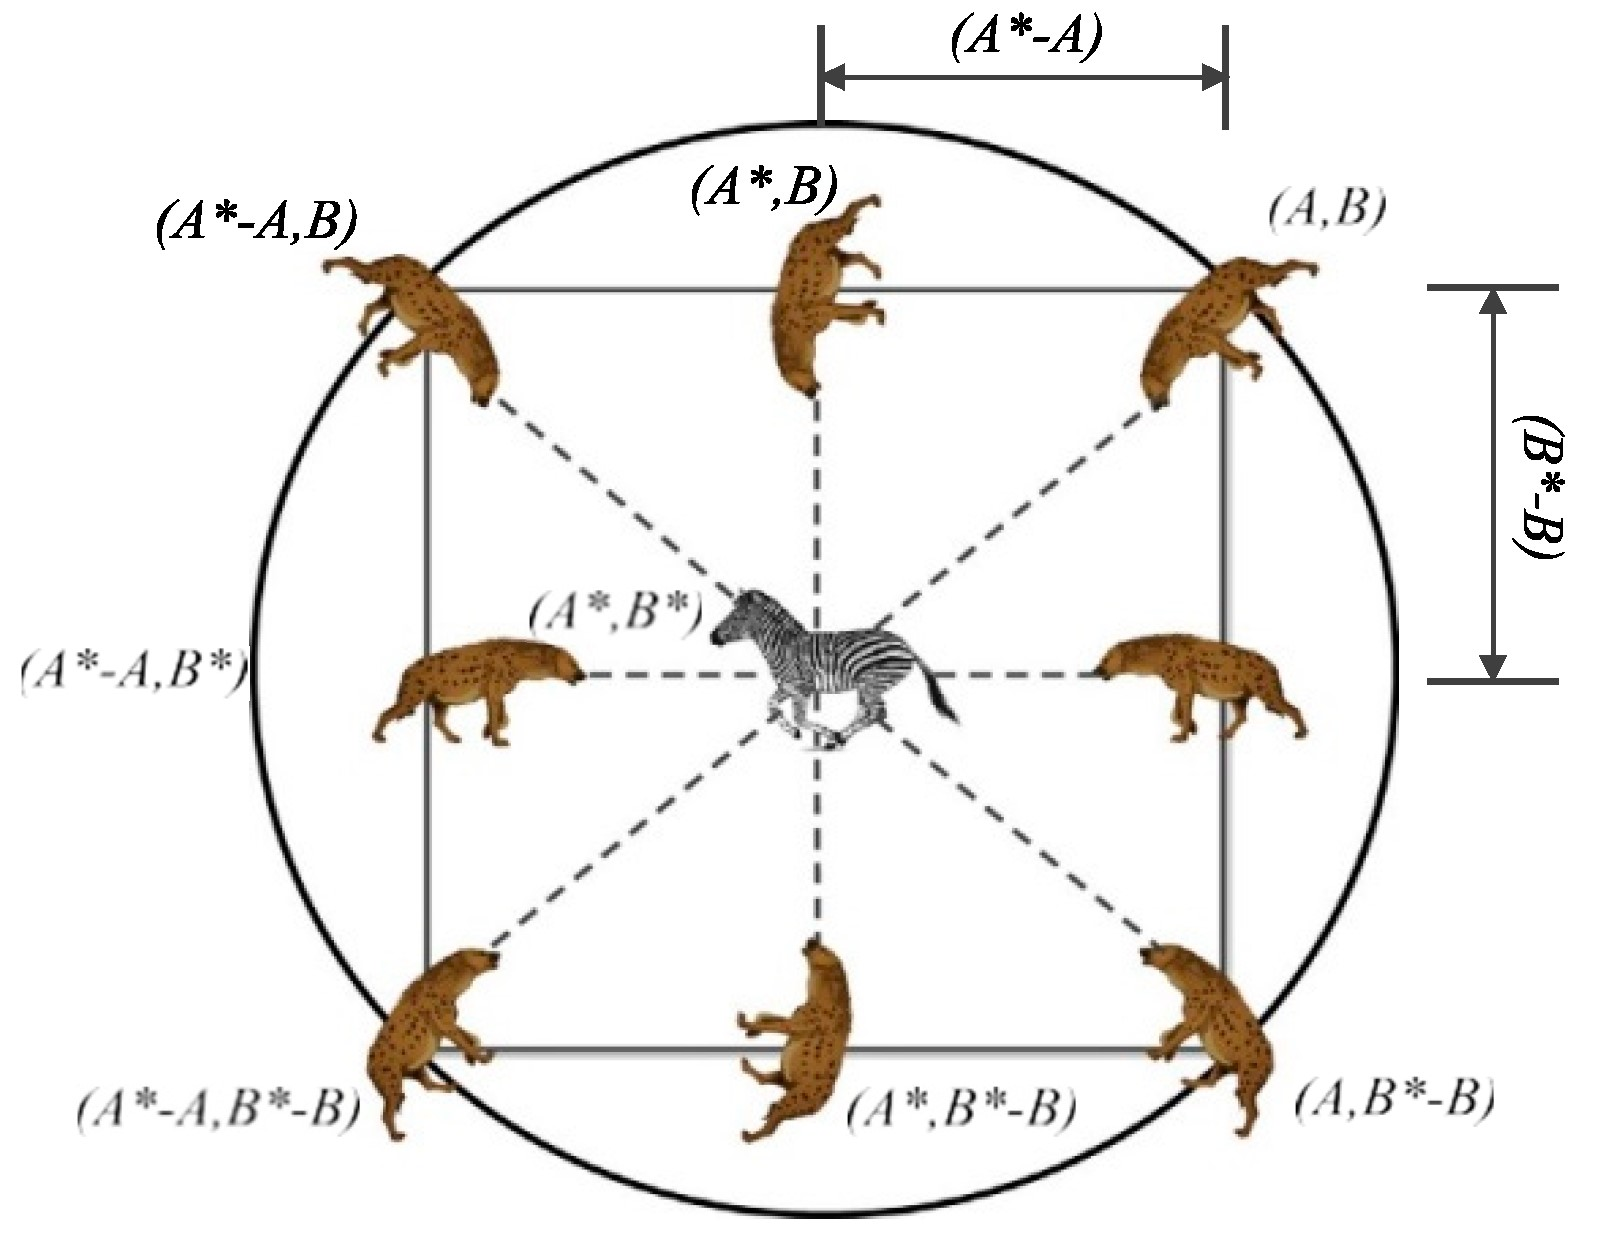
\includegraphics[width=0.8\textwidth]{F1_SHO_circling.jpg}
  \caption{Position vectors of spotted hyena in 2D before attacking the prey}
\end{figure}


We count how many perfect spots there are in the bunch when they go hunting. This count depends on something called the coefficient vector E and is given by

\begin{equation}
    \overrightarrow{D}_h = \overrightarrow{B}\bullet \overrightarrow{P}_h-\overrightarrow{P_k}
\end{equation}

\begin{equation}
    \overrightarrow{P}_k = \overrightarrow{P_h}\bullet \overrightarrow{E}.\overrightarrow{D_h}
\end{equation}

\begin{equation}
    \overrightarrow{C}_h = \overrightarrow{P}_k + \overrightarrow{P}_{k+1}+ .... + \overrightarrow{P}_{k+N}
\end{equation}

Here Pk shows where the spotted hyenas are, and "Ph" points to the very best spot where a spotted hyena can be found. The letter "N" tells us how many spotted hyenas there are, and we can count them as follows:
\begin{equation}
    N  = count_{nos}(\overrightarrow{P}_h + \overrightarrow{P}_{h+1}+ .... + (\overrightarrow{P}_{h}+\overrightarrow{M}))
\end{equation}


In this situation, we have a vector called 'M' that's randomly set between 0.5 and 1. Equation 8 represents a bunch of the best solutions, like a team of hunters. When these hunters get really close to their target, we use a special number called 'E' to decide if they should attack. If 'E' is less than 1, it means they go in for the kill. This attack on the target is shown in math as follows:

\begin{equation}
    \overrightarrow{P_{x+1}}= \overrightarrow{C_h}/N 
\end{equation}


In the formula, $P_{x+1}$ 
is to figure out where the best solution is and how the other search entities should move based on where the best one is. 
In the SHO algorithm, we keep track of the best solution and update the positions of other search entities based on where this best solution is. We stop the algorithm when a specific condition is met. 
So whole process can be understood by following the steps:

\textbf{1) Initialize Population:} Begin by creating a population of spotted hyenas (search agents) labeled as Pi, where i ranges from 1 to n.
ested on five constrained and one unconstrained
engineering design problems: welded beam,
tension/comp

\textbf{2) Set Initial Parameters:} Choose the initial parameters for the SHO algorithm, including h, B, E, and N. also mention no of iterations.

\textbf{3) Evaluate Fitness:} Calculate the fitness value for each search agent to assess their performance.

\textbf{4) Explore Best Agent:} Identify the best-performing search agent within the search space.

\textbf{5) Define Optimal Group:} Define a group of optimal solutions or clusters using Eq 8,9  until good results.

\textbf{6) Update Agent Positions:} Update the positions of the search agents using Equation (10).

\textbf{7) Boundary Checking:} Ensure that no search agent goes beyond the defined boundaries in the search space. Adjust their positions if needed.

\textbf{8) Update Fitness and Optimal Solution:} Calculate and update the fitness values of the search agents. If a better solution than the previous optimal one is found, update the vector Ph.

\textbf{9) Update Spotted Hyena Group:} Update the group of spotted hyenas, Ch, with the updated fitness values of the search agents.

\textbf{10) Check Stopping Criteria: }Check if the algorithm's stopping criterion has been met. If satisfied, stop the algorithm; otherwise, return to Step 5 i.e. Define Optimal Group.

\textbf{11) Optimal Solution: } As after stopping criteria is satisfied, return the best optimal solution whichever obtained so far.


To solve an optimization problem using the Spotted Hyena Optimizer (SHO) algorithm (\cite{dhiman2017spotted}) :


\begin{algorithm}
\caption{Spotted Hyena Optimizer}\label{alg:cap}
\textbf{Input:} Population Pi the spotted hyenas (i = 1, 2, . . ., n)\\
\textbf{Output:} Best hyena\\\\
\text{\textbf{procedure } SHO}\\
\text{Initialize parameters h, B, E, and N}\\
\text{Calculate the fitness of each hyena.}\\
\text{Set the $P_h$ = best hyena with lowest fitness value }\\
\text{Initialize the cluster $C_h$ = cluster of far-optimal solutions to be empty. }\\
\text{\textbf{\hspace{0.5cm} while} ($x < Max Iterations$) }{\textbf{do}\\
\text{\textbf{\hspace{0.9cm} for} each hyena : }\\
\text{\hspace{1.5cm}By using Eq. (10) update position of hyena}\\
\text{\hspace{1cm}\textbf{end for}}\\
\text{\hspace{1cm}Update the paramters of SHO}\\
\text{\hspace{1cm}Boundry check for search Hyenas and adjust it}\\
\text{\hspace{1cm}Calculate the fiteness for each hyena}\\
\text{\hspace{1cm}Update Ph for better solution}\\
\text{\hspace{1cm}Update the cluster $C_h$ by using Ph}\\
\text{\hspace{1cm}x = x+1}\\
% \EndWhile\\
\text{\textbf{\hspace{0.5cm} end while}}\\
\text{return Ph}\\
\text{\textbf{end procedure}}}
\end{algorithm}

The overall time complexity of the SHO algorithm is O(k × n × Maxiter × dim × N) and the total space complexity is O(n × dim). 'n' determines many times random group is created. This group is based on how many search agents there are and the lowest and highest values allowed in a test problem. 'dim' tells us how many aspects we're checking and fixing in the solutions if they go outside the allowed space. Maxiter is maximum iterations and N is the count of spotted hyenas.


\section{Results}

The SHO algorithm is effective in solving a variety of optimization problems, including engineering design problems, scheduling problems, and financial optimization problems. It is robust to noise and outliers. It is easy to implement and tune. 
The SHO algorithm is competitive with other metaheuristic algorithms, such as the Particle Swarm Optimization algorithm and the Genetic Algorithm.
This section explains how we tested the new algorithm. Proposed paper used 29 standard test problems to see how well SHO algorithm works. These test problems are explained in Section 3. Then, we looked at the results and compared them to eight other commonly used methods to see how good our algorithm is.

\subsection{Benchmark test comparison and analysis}
The given algorithm was evaluated on total of 29 benchmark functions, which were divided into four categories: unimodal, multimodal, fixed-dimension multimodal, and composite functions. The unimodal functions have one global optimum, while the multimodal functions have multiple local optima. The fixed-dimension multimodal functions are a subset of the multimodal functions that have a fixed number of dimensions. The composite functions are a combination of classical functions.



The proposed algorithm was compared to eight other well-known algorithms: Particle Swarm Optimization (PSO) (\cite{kennedy1995particle}), Grey Wolf Optimizer (GWO) (\cite{mirjalili2014grey}), Sine Cosine Algorithm (SCA) (\cite{mirjalili2016sca}), etc. So total search agents for each algorithm was given a value 30.
The outcomes for functions F1 to F29 indicate that the SHO algorithm performs exceptionally well when compared to other optimization methods. To dig deeper into how good this new algorithm is, we're going to take a closer look at how it tackles six classic engineering design problems in the upcoming sections.
Further Convergence analysis and Scalability studies are performed and results was favourable. Statistical testing proves that This algorithm is significant statistically when compared with other algorithms.

\subsection{SHO for engineering problems}
SHO is a robust, easy to implement algorithm, hence if you are facing an engineering problem that needs to be solved, SHO is a potential algorithm to consider.
In this section, the SHO algorithm was tested on five constrained and one unconstrained engineering design problems: welded beam,speed reducer,pressure vessel etc.  So different penalty functions to handle constraint problems.
Various standard engineering problems like Tension/compression spring design problem, Pressure vessel design, Speed reducer design problem, Rolling element bearing design problem,  Displacement of loaded structure are optimized with SHO and mostly it outperformed other algorithms. 
The results showed that the proposed algorithm outperformed the other algorithms on all four categories of benchmark functions. The proposed algorithm was able to find the global optimum of the unimodal functions in fewer iterations than the other algorithms. The proposed algorithm was also able to find the global optimum of the multimodal functions, even when the functions had multiple local optima. (\cite{dhiman2017spotted,dhiman2018multi,dhiman2019spotted})
We have implementated the SHO for optimizing two types of problems, the first one is minimizing the value of the given function and second one is to parameter tunning for machine learning classification models.
% The a standard engineering problem of Welded beam design is solved with other  algorithms too. The goal of this problem is to minimize the fabrication cost of a welded beam. There are four optimization variables in this problem:

% clamped bar's length (l), weld thickness (h),  bar height (t), bar's thickness (b)

% The comparision  table is given as : 

% \begin{table}[h]
%     \centering
%     \captionsetup{font=it}
%     \caption{results for welded beam design by many algorithms.}
%     \label{tab:example}
%     \begin{tabularx}{\textwidth}{|Y|Y|Y|Y|Y|Y|}
%     \hline
%     \textbf{Algorithms} &  \textbf{h} & \textbf{t}  &  \textbf{h} & \textbf{b} & \textbf{Optimum cost by using Algo}\\
%     \hline
%     SHO & 0.20573 & 3.47484 & 9.035799 & 0.205811 & \textbf{1.725661} \\
%     \hline
%     GWO & 0.205688 & 3.47540 & 9.036964 & 0.206229 & 1.726995\\
%     \hline
%     PSO & 0.197411 & 3.31506 & 10.00000 & 0.201395 & 1.820395\\
%     \hline
%     GSA & 0.147098 & 5.49074 & 10.00000 & 0.217725 & 2.172858\\
%     \hline
%     GA & 0.164171 & 4.03254 & 10.00000 & 0.223647 & 1.873971\\
%     \hline
%     HS & 0.206487 & 3.63587 & 10.00000 & 0.203249 & 1.836250\\
%     \hline
%     \end{tabularx}
% \end{table}
\subsubsection{Minimizing the cost of the objective function: }
We have taken a following function f(x) and applied SHO algorithm to find the smalled value and position of x in the search space. 

\begin{equation}
    f(x) = cos(3x)+ 3.sin(3x)) + x^2
\end{equation}

The SHO algorithm worked well and converges to find the optimal solution. We also tried to find the optimized answer with the help of Particle Swarm Optimization Algorithm (PSO). The figure 2 and figure 3 shows the performaces of both the algorithms. 
Figure 2 showcases the fiteness of the standard objective function named F292017 (\cite{thieu_nguyen_2020_3711682}) to be minimize whereas Figure 3 shows the results of optimization of Eq. (11). As plot from figure 3 suggest that for easy linear problem SHO is as good as PSO as both converges quickly. But Figure 2 shows that when complexity of problem increases SHO converges faster than PSO to the best optimal solution. 
So SHO works well in this type of problems and outperforms other algorithms.

\begin{figure}
  \centering
      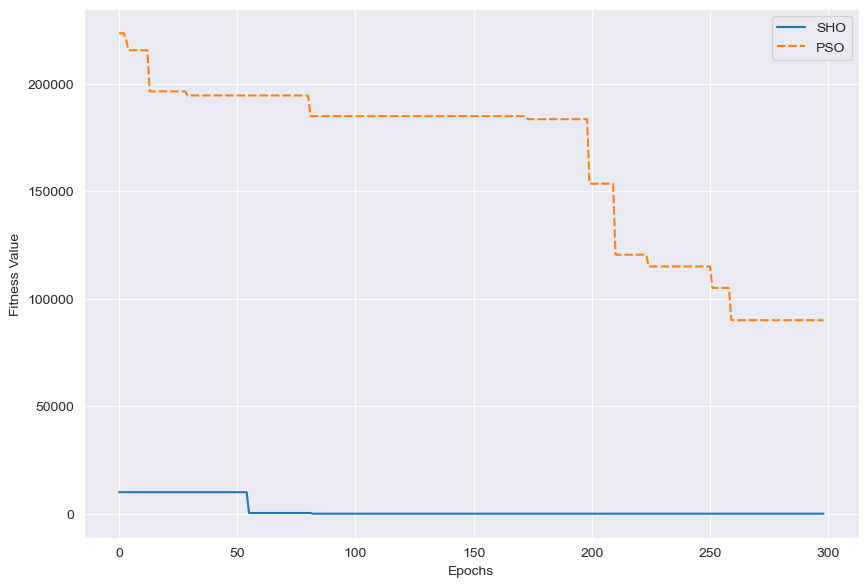
\includegraphics[width=0.9\textwidth]{F4_F29_data_fitness.png}
  \caption{Results of optimization of F292017 data instance}
\end{figure}

\begin{figure}
  \centering
      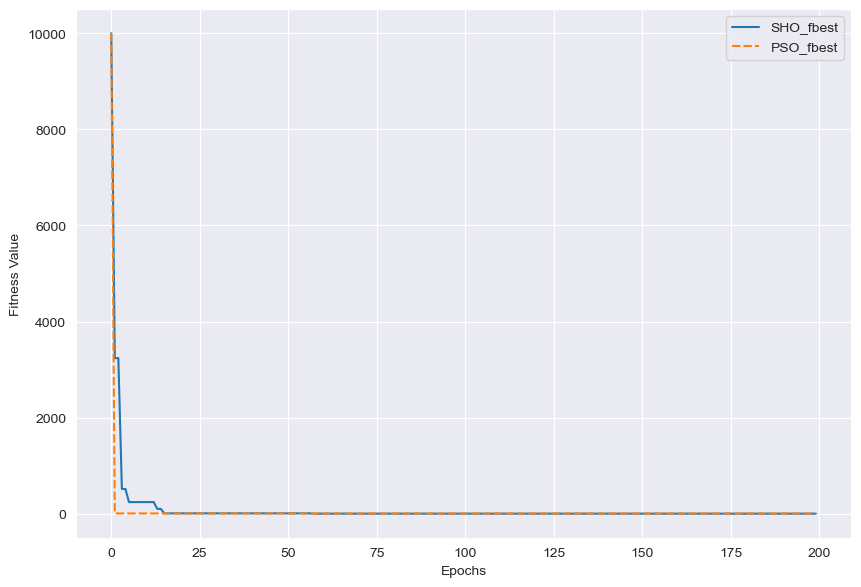
\includegraphics[width=0.9\textwidth]{F5_Self_d_question_fitness.png}
  \caption{Results of optimization of self define function}
\end{figure}

\subsubsection{Hyperparameter tunning with SHO: } We used SHO algorithm to find the best combination of the hyperparameter of the classifiers.
For that sake we take many datasets from small size (less than 200 data points) to higher size (More than 1 lakh datapoints). We used two different classification models as follows:  KNN and LGBM CLassifier. We have analyse the performance of the alogorithms given by the log\_loss of the classifier.
In this case PSO seems to be more optimal than the SHO algorithm. We tried to increase the complexity of the problem for which PSO works far well than SHO. Hence we can say that for smaller datasets SHO can work well for finding the right combination of the hyperparametrs, but as the complexity increases its getting hard towards getting optimized. This may change in respect of the data dependency of classification model, data size, number of iterations etc. .
So results suggest that hyperparameter parameter tunning can done by SHO but other algorithm can outperform SHO for the same task for complex problems. 

\section{Conclusion}
This paper presented a Spotted Hyena Optimizer (SHO) in a simple terms. 
The Spotted Hyena Optimizer (SHO) algorithm is a novel metaheuristic algorithm that is inspired by the hunting behavior of spotted hyenas. The SHO algorithm has been shown to be effective in solving a variety of optimization problems, including minimizing the value of a given function and parameter tuning for machine learning classification models.
The results of the study showed that the SHO algorithm was able to find the optimal solution to the function minimization problem in a relatively short amount of time. The SHO algorithm also outperformed the Particle Swarm Optimization (PSO) algorithm on this problem.
The results of the study also showed that the SHO algorithm was able to find the optimal hyperparameters for machine learning classification models. However, the PSO algorithm was able to find better hyperparameters for some datasets. This may be because the PSO algorithm is more sensitive to the hyperparameters of the classification model.
Overall, the results of the study suggest that the SHO algorithm is a promising new metaheuristic algorithm that can be used to solve a variety of optimization problems. The SHO algorithm is more efficient than other metaheuristic algorithms such as the PSO algorithm for function minimization problems. However, the PSO algorithm may be more effective for parameter tuning for machine learning classification models.
We believe that the SHO algorithm is a significant contribution to the field of metaheuristic optimization. We hope that this paper will help to promote the use of the algorithm and encourage further research in this area.

\clearpage % To force all figures before references
\printbibliography % For APA or IATBR custom citation style
\end{document}